\clearpage
\chapter{\textbf{Vorwissen}}\label{chap:Vorwissen}
\addtocontents{toc}{\vspace{0.8cm}}
Im Folgenden werden ein paar grundsätzliche Sachverhalte und Definitionen festgelegt und erläutert. Sie sollen das Verständnis der Algorithmen in Kapitel \ref{chap:Lokalisierung - Lösungsansätze} ermöglichen und fördern. 


\section{bestimmbare Positionen}\label{sec:bestimmbare Positionen}
\addtocontents{toc}{\vspace{0.8cm}}
Die Position eines sich auf dem Boden bewegenden mobilen Roboters, in Bild \ref{fig:1a_dd}  eines sog. Differential Drive Roboters, kann angegeben werden durch 
$p=\mathbf{\begin{psmallmatrix}
x & y & \psi
\end{psmallmatrix}}^\intercal$.
Hierbei bezieht sich $x$ auf die Position gepeilt auf die x-Achse, $y$ die Position gepeilt auf die y-Achse und $\psi$  den Winkel zwischen der Ausrichtung des Roboters und der x-Achse. Die Literatur bezeichnet die erhaltene Position im Fall eines bodengebundenen Roboters als eine 2D Position.\\
Zur Positionsbestimmung eines UAVs kommt im Falle einer 3D Positionsbestimmung eine weitere Achse hinzu, sodass die 3D Position angegeben werde kann durch
$p=\mathbf{\begin{psmallmatrix}
x & y & z & \psi
\end{psmallmatrix}}^\intercal$.
Die zusätzliche Variable $z$ bezeichnet hierbei die Position des Roboters gepeilt auf die z-Achse. (siehe Bild \ref{fig:1b_uav})\\
Eine weitere Darstellung der Position eines UAVs ist die 6D Position. Hierbei kommen zu der eben besprochenen 3D Position zwei Winkel hinzu, wodurch die 6D Position angegeben werden kann durch
$p=\mathbf{\begin{psmallmatrix}
x & y & z & \psi & \theta & \varphi
\end{psmallmatrix}}^\intercal$.
Dies folgt einer Konvention der Luft-und Raumfahrt, dem Schiffbau und dem Automobilbau \cite{website:cosmos-indirekt}, wonach die Reihenfolge der Eulerschen Winkel in Gier-, Nick-, und Rollwinkel (engl. \textit{yaw, pitch, roll}) festgelegt ist. (siehe Bild \ref{fig:1c_euwinkel}) Der Winkel $\psi$ beschreibt folglich den Gierwinkel, $\theta$ den Nickwinkel und $\varphi$ den Rollwinkel.\\

% Koordinatensystemsbilder für Positionen
\mbox{}
\begin{figure}
  \begin{subfigure}{.3\textwidth}
    \centering
    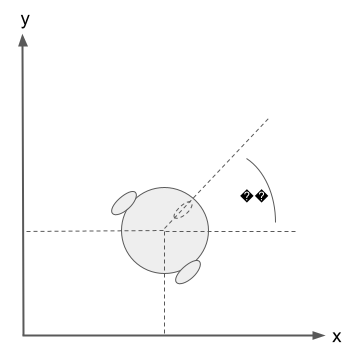
\includegraphics[width=.8\linewidth]{pic/vorwissen/1a_diffdrive.png}
    \caption{Position eines \textit{Differential Drive} Roboters}
    \label{fig:1a_dd}
  \end{subfigure}\hfill
  \begin{subfigure}{.3\textwidth}
    \centering
    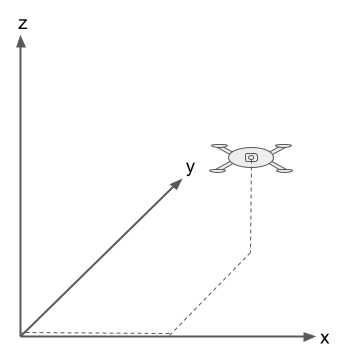
\includegraphics[width=.8\linewidth]{pic/vorwissen/1b_uav.png}
    \caption{Position eines UAV im dreidimensionalen Raum}
    \label{fig:1b_uav}
  \end{subfigure}\hfill
  \begin{subfigure}{.3\textwidth}
    \centering
    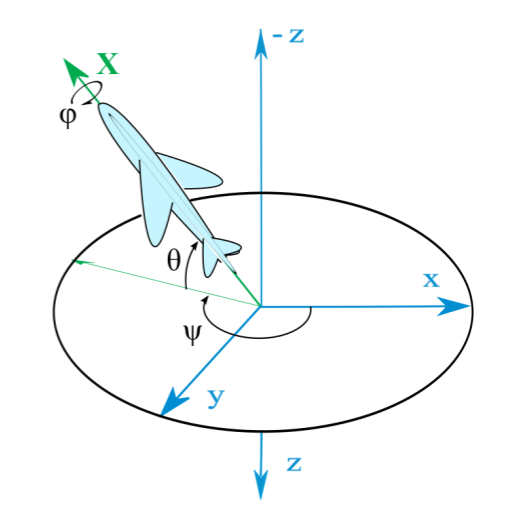
\includegraphics[width=.8\linewidth]{pic/vorwissen/1c_eulerwinkel.png}
    \caption{Konvention für Eulersche Winkel \cite{website:cosmos-indirekt-grafik}}
    \label{fig:1c_euwinkel}
  \end{subfigure}
  \label{fig:positionen}
\end{figure}
\mbox{}


\section{Sensorik}\label{sec:Sensorik}
\addtocontents{toc}{\vspace{0.8cm}}
Die Sensorik eines mobilen Roboters kann unterteilt werden in interne- und externe Sensoren. Die internen Sensoren befinden sich innerhalb des Systems, und umfassen meistens Beschleunigungs-, Gyro- und gegebenenfalls Magnetometer Sensoren, welche für gewöhnlich in einer sogenannten \textit{Internal Measurement Unit} (IMU) zusammengefasst werden. Sie können genutzt werden, um ohne Wissen über die Außenwelt Aufschluss über die Position des Roboters über die Zeit zu geben. Dies wird auch als \textit{dead reckoning} bezeichnet, da sich die aktuelle Position nur aus der letzten errechneten Position errechnen lässt, welche bereits fehlerbehaftet sein kann. Da die Messung eines Sensors immer mit Messfehlern behaftet sein kann, wird auf diese Messung eine Art Toleranzbereich mit Wahrscheinlichkeitsverteilung angewendet, die oft einer Gaußschen Normalverteilung entspricht. (siehe Bild 3a) Dadurch wird die Unsicherheit bzw. der Drift beim dead reckoning größer, je länger sich der Roboter ohne Berichtigung durch äußere Messungen fortbewegt. (siehen Bild 3b)\\
Zu eben dieser Berichtigung durch äußere Messungen werden die externen Sensoren eingesetzt. Sie erfassen die den Roboter umgebende Welt durch beispielsweise Kameras, Ultraschallsensoren oder Laser-Range-Scanner. Auch die durch diese Sensoren gesendeten Messung können Messfehler enthalten, weswegen die Messungen wie die der internen Sensoren mit einem Toleranzbereich, dargestellt durch eine Wahrscheinlichkeitsverteilung, verrechnet werden.\\

[Bilder 3a, 3b einfügen]

\section{\textit{Motion-Model}}\label{sec:Motion-Model}
% TODO Motion-Model schreiben
hier wird bald was über das motion-model stehen

\section{\textit{Observation-Model}}\label{sec:Observation-Model}
% TODO Observation-Model
hier wird bald was über das observation-model stehen.



\section{Kartenrepräsentation}\label{sec:Kartenrepräsentation}
\addtocontents{toc}{\vspace{0.8cm}}
Zur Positionsbestimmung in einer Karte ist die Auswahl der Kartenrepräsentation maßgebend. In der Kartendarstellung wird unterschieden zwischen einem topologischen- und einem metrischen Gerüst für eine Karte.\\
Bei einem topologischen Rahmen werden nur die Orte und dessen Beziehungen berücksichtigt, sodass die Karte ein Graph ist, bestehend aus Knoten, die die Orte repräsentieren und Bögen, die die Verbindungen der Orte darstellen. In einem metrischen Gerüst für eine Karte wird die räumlich-, Koordinatensystem-basierte Darstellung der Karte verwendet. Die Objekte innerhalb der Karte haben hierbei genaue Koordinaten.\\
Die in dieser Arbeit zumeist verwendeten Karten nutzen sogenannte \textit{Occupancy Grid Maps}. Hierbei wird ein Gitter mit definierter Masche auf die Karte gelegt. Befindet sich ein Objekt in der Karte, so wird jedes Gitterkästchen in dem sich das Objekt befindet als besetzt (engl. \textit{occupied}) gewertet und wie in Bild 2 schwarz eingefärbt. So können die für eine Karte benötigten Datenmengen kontrolliert und eingegrenzt werden.\\
Im dreidimensionalen Raum können Occupancy Grid Maps ebenfalls eingesetzt werden. Der Raum kann dann nicht mehr nur mithilfe von zweidimensionalen Kästchen diskretisiert werden, sondern muss durch Würfel, sogenannte \textit{Voxel} eingeteilt und dargestellt werden.\\

% TODO Occupancy Grid Map Bilder hinzufügen
[Bild 2 einfügen]
